\chapter{Arquitechture}
\label{chap:architecture}

\begin{chapterintro}

In this section, we describe the overall architecture of a QA system that features social dialog in a learning environment.
 
\end{chapterintro}

\cleardoublepage

\section{Overview}

As already stated, in this section we will describe the arquitechture of our system, starting with the modules identified in the requirements. This requirements are:
\begin{enumerate}[noitemsep, label=(\roman*)]
 \item Present the user with a simple interface for their questions, and to present them with the answers.
 \item Classify each input according to the speech act it performs.
 \item Track dialog options according to the speech.
 \item Implement a QA system being able to search the document library and extract a short answer.
 \item Extend the documents library, scrapping external documents and producing semistructures indexes.
 \item Follow up the learning process, and use it to improve the learning experience. 
\end{enumerate}

In figure \ref{fig:arch1} we show the global architecture of the system, identifying four main modules: Conversational Agent, Teaching Agent, Question Answering and Information Extraction Agent. In the rest of this chapter we will discuss the function of reach module.

\color{red}\emph{Añadir info sobre el clasificador?}\color{black}


\begin{figure}[!htbp]
    \centering
    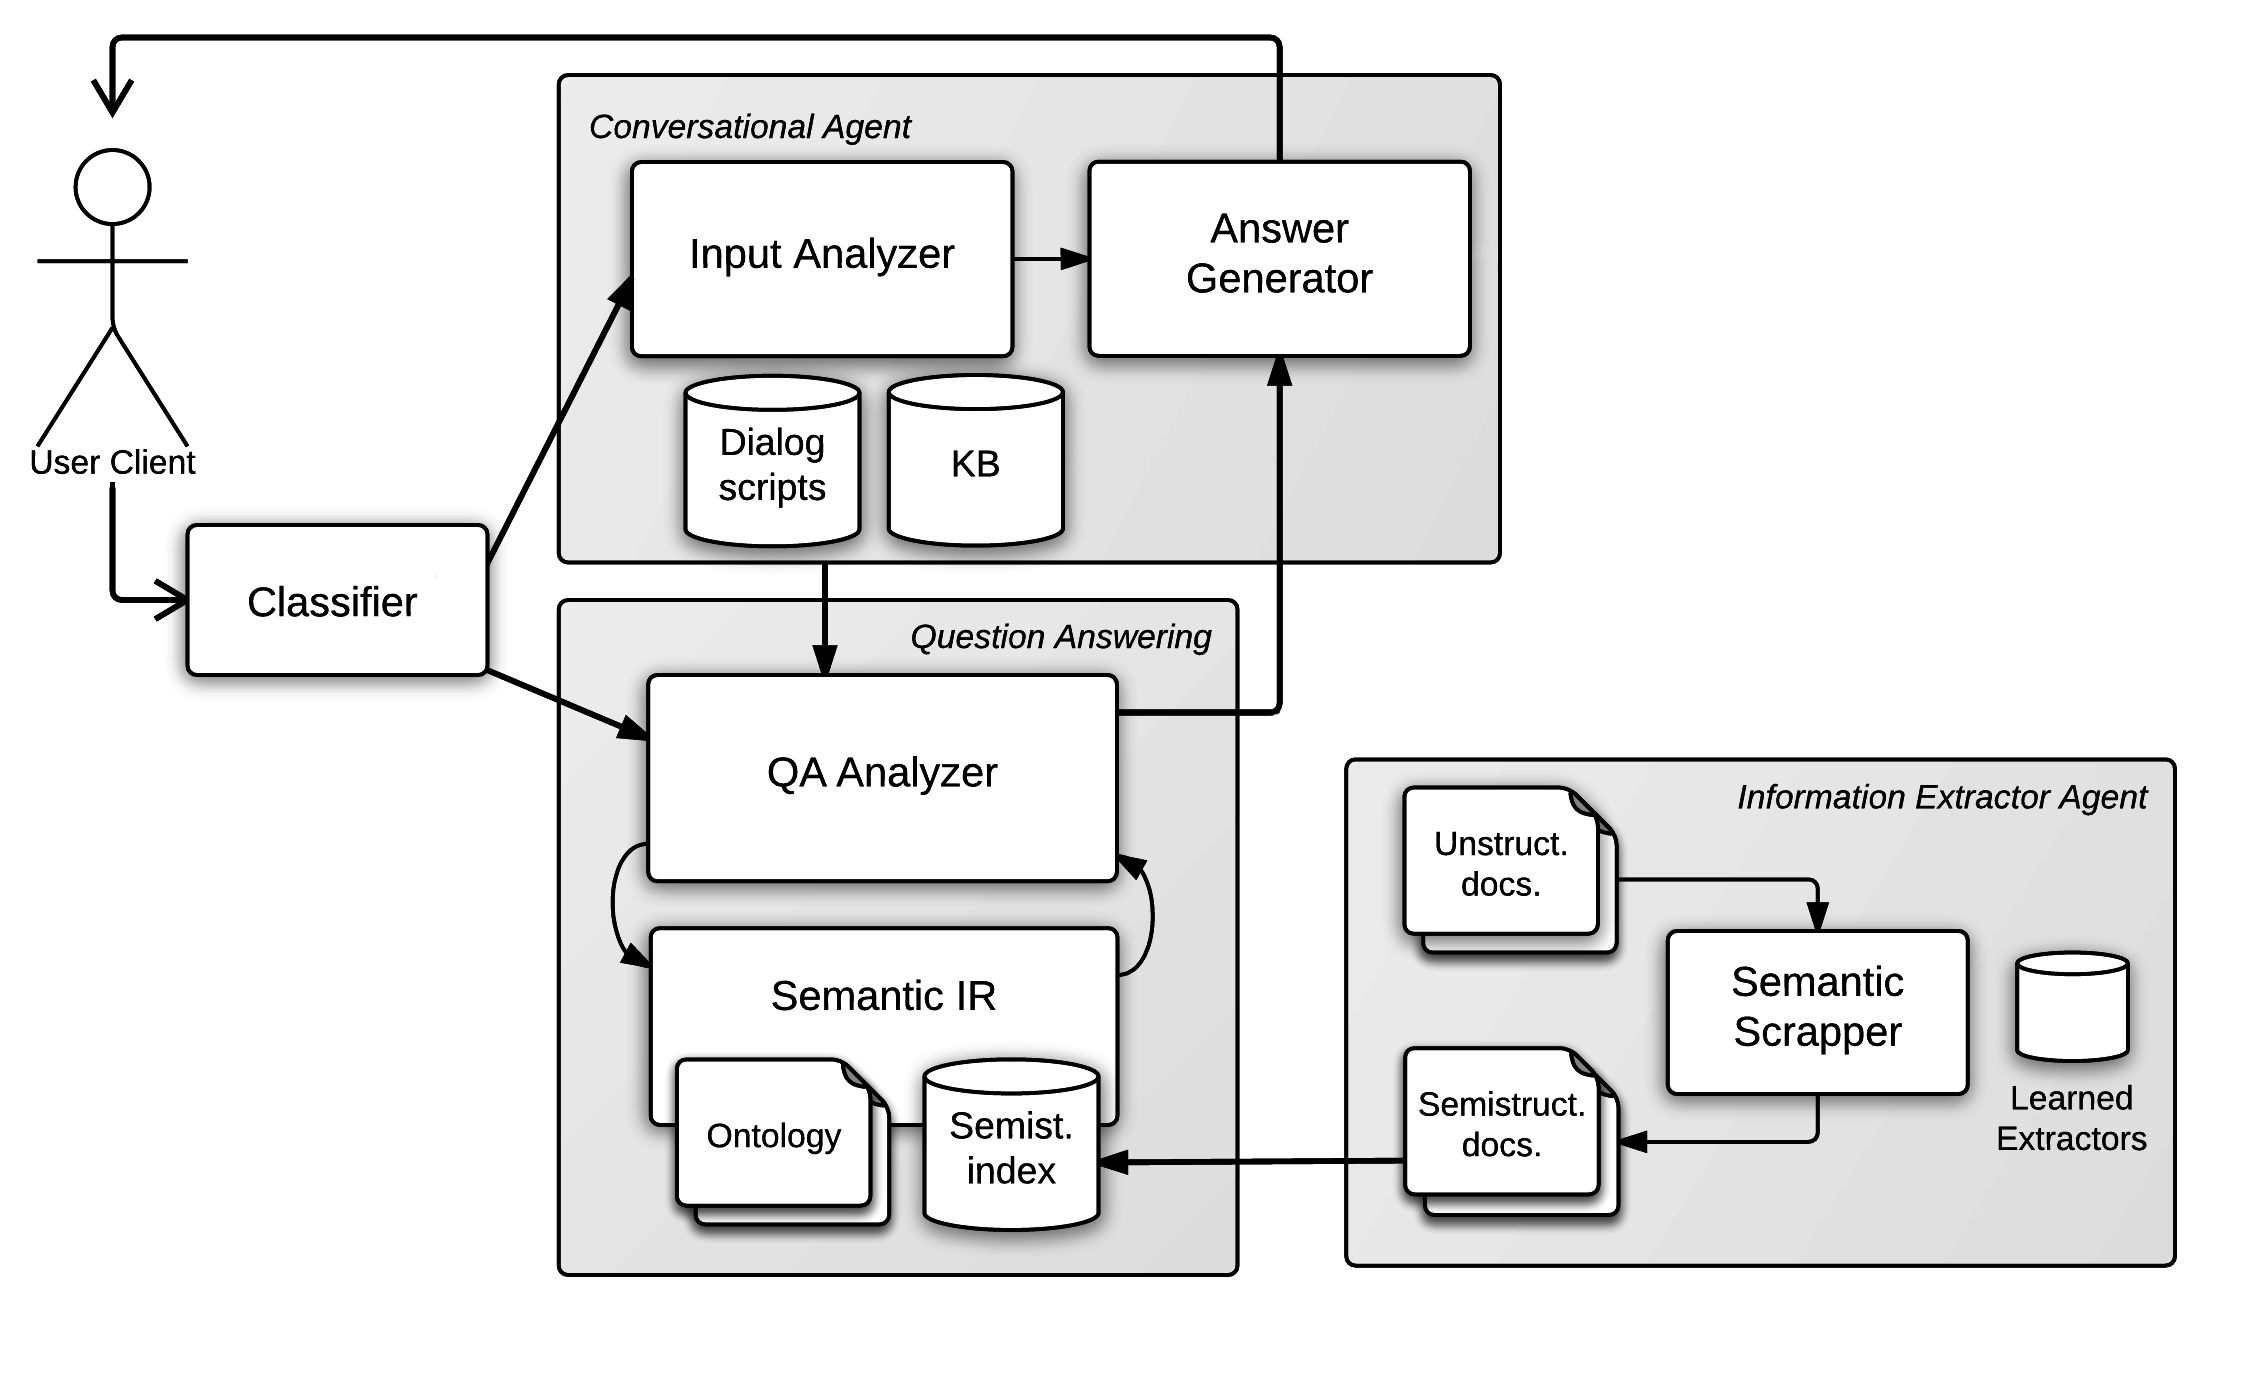
\includegraphics[width=0.7\textwidth]{img/arch/global_1-3.png}
    \caption{Global view of the architecture proposed}
    \label{fig:arch1}
\end{figure}

\section{Conversational Agent}

\section{Question Answering}

\section{Information Extractor}

\section{Teaching agent}